\section{System Architecture}
\label{sec:system_architecture}

Chatnalyxer is composed of three loosely coupled microservices: an Edge Ingestion Layer, a Processing Core, and a Storage/Scheduling Layer. Separating these concerns is not merely an organizational preference—it is an architectural necessity dictated by the latency and throughput constraints of real-time messaging environments (illustrated in Fig.~\ref{fig:sys_arch}).

\begin{figure*}[tbp]
    \centering
    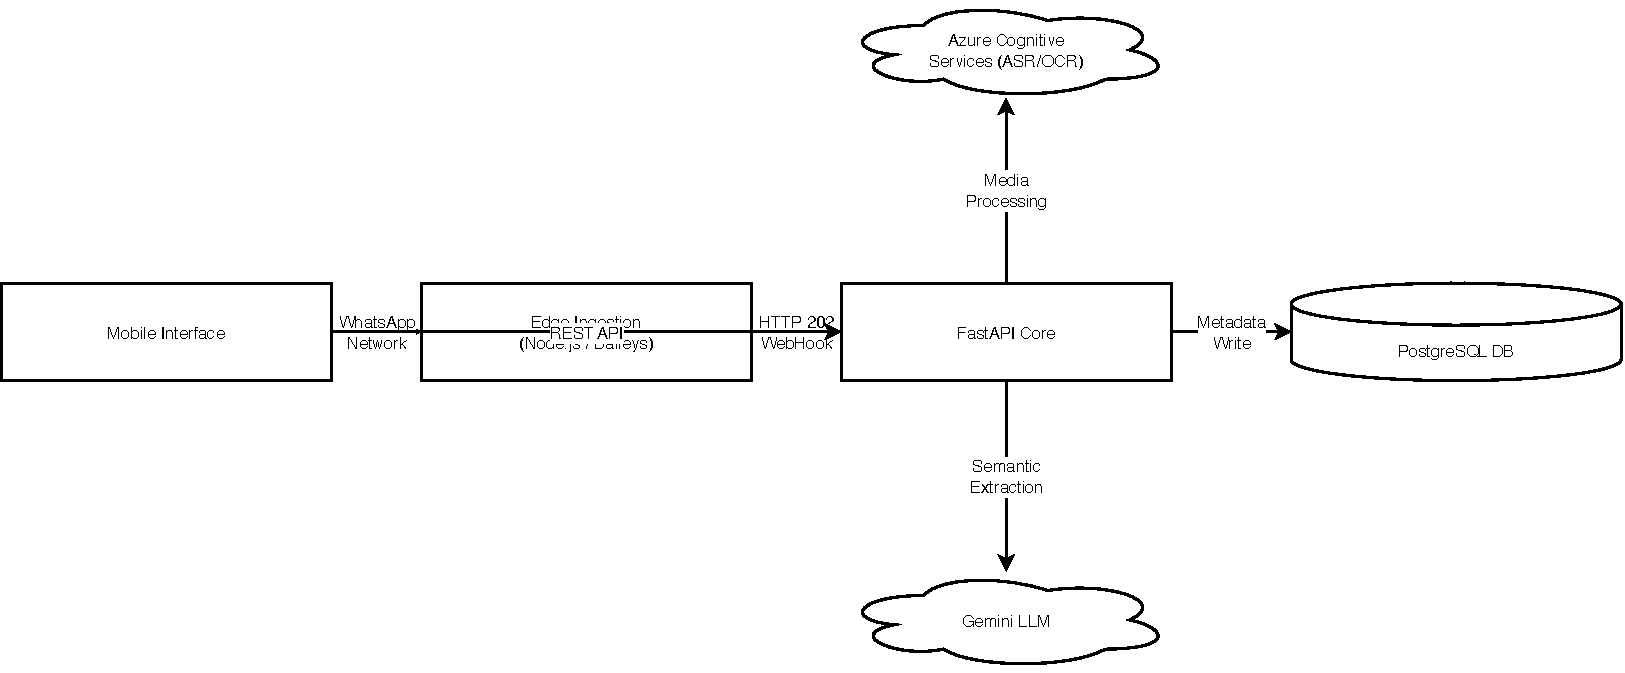
\includegraphics[width=0.85\textwidth,keepaspectratio]{figures/Fig1_System_Architecture.pdf}
    \setlength{\abovecaptionskip}{4pt}
    \setlength{\belowcaptionskip}{-4pt}
    \caption{High-level system architecture of the Chatnalyxer pipeline. The Node.js edge ingestion layer is asynchronously decoupled from the FastAPI processing core via an HTTP 202 WebHook, bounding local ingestion latency to $\mathcal{O}(1)$ under burst traffic conditions.}
    \label{fig:sys_arch}
\end{figure*}

\subsection{The HTTP 202 Asynchronous Decoupling Boundary}
A na\"ive implementation of this pipeline would process each incoming message synchronously: the edge layer receives a WebSocket event, invokes the LLM API, waits for the response (typically 1--3 seconds), and only then acknowledges the message. Under Poisson-distributed burst traffic, this approach quickly exhausts the Node.js connection pool, causing dropped messages. This is not a theoretical concern—it is the failure mode of all synchronous chat-bot architectures under moderate load.

Chatnalyxer avoids this through an HTTP 202 design pattern. When the Node.js edge layer forwards a payload to the FastAPI core, the core immediately spawns an \texttt{asyncio} background coroutine and returns \texttt{HTTP 202 Accepted}. The edge layer is free to process the next incoming event before the initial inference has completed. This decouples ingestion throughput from inference latency, bounding the edge-side processing time to $\mathcal{O}(1)$—consistently measured at under 15 ms—regardless of LLM response time.

\subsection{Processing Core and Ephemeral Architecture}
A persistent concern with any system that passively monitors private conversations is data retention. To address this, the Processing Core operates on a strictly ephemeral memory model: raw message payloads, images, and audio are held exclusively in volatile RAM during the inference window. Once structured metadata has been written to PostgreSQL, the raw content is immediately deallocated. No chat histories are written to disk at any stage in the pipeline.

\subsection{Scalability Analysis}
The microservice architecture was designed explicitly for horizontal scaling. The FastAPI core is stateless; deploying behind a round-robin load balancer enables processing of an arbitrary number of concurrent webhook events. In stress tests, a single T4 GPU instance handled peaks of 50 messages per second. At enterprise scale—e.g., 10,000 active users generating 1 million messages daily—the PostgreSQL metadata storage layer scales efficiently due to the minimal footprint of extracted tasks (approximately 250 bytes per row). The primary bottleneck at this scale shifts from local compute to cloud API rate limits, which can be mitigated via provisioned throughput or rotating API keys.
